\documentclass[a4paper,12pt]{article}
\usepackage[left=1in,right=1in,top=0.85in,bottom=1.15in]{geometry}
\usepackage{multicol}
\usepackage{enumitem}
\usepackage{titlesec}
\usepackage{background}
\usepackage{fancyhdr}
\usepackage{graphicx}
\setlist[itemize]{noitemsep, topsep=0pt}
\titlespacing*{\section}{0pt}{1.2ex}{0.5ex}

\newcommand{\dkflag}{%
    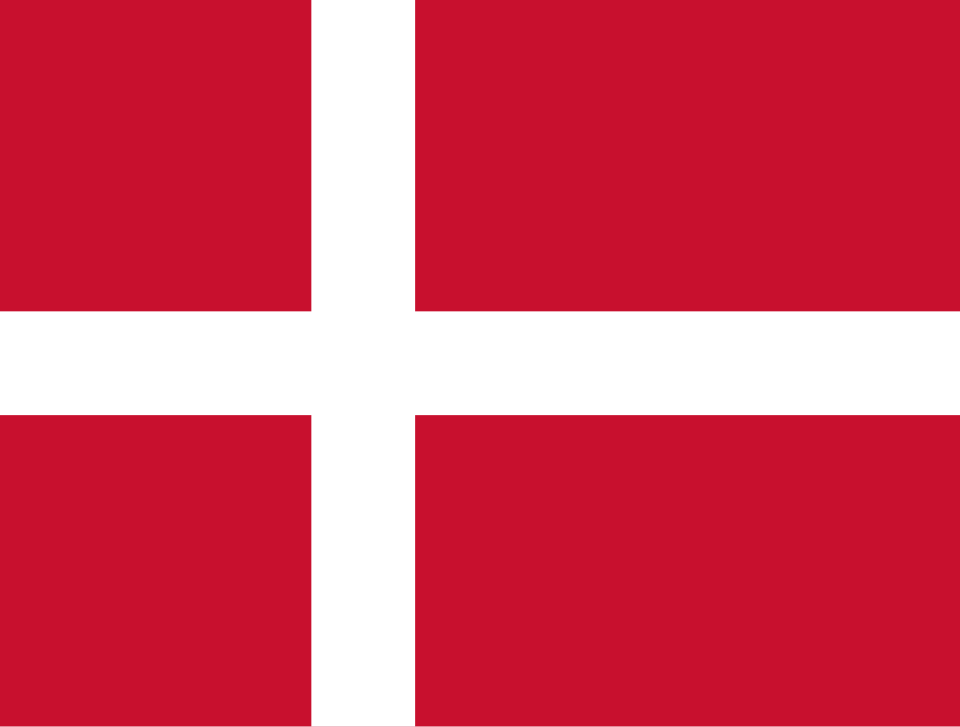
\includegraphics[height=.9em]{denmark.png}%
}

\newcommand{\ukflag}{%
    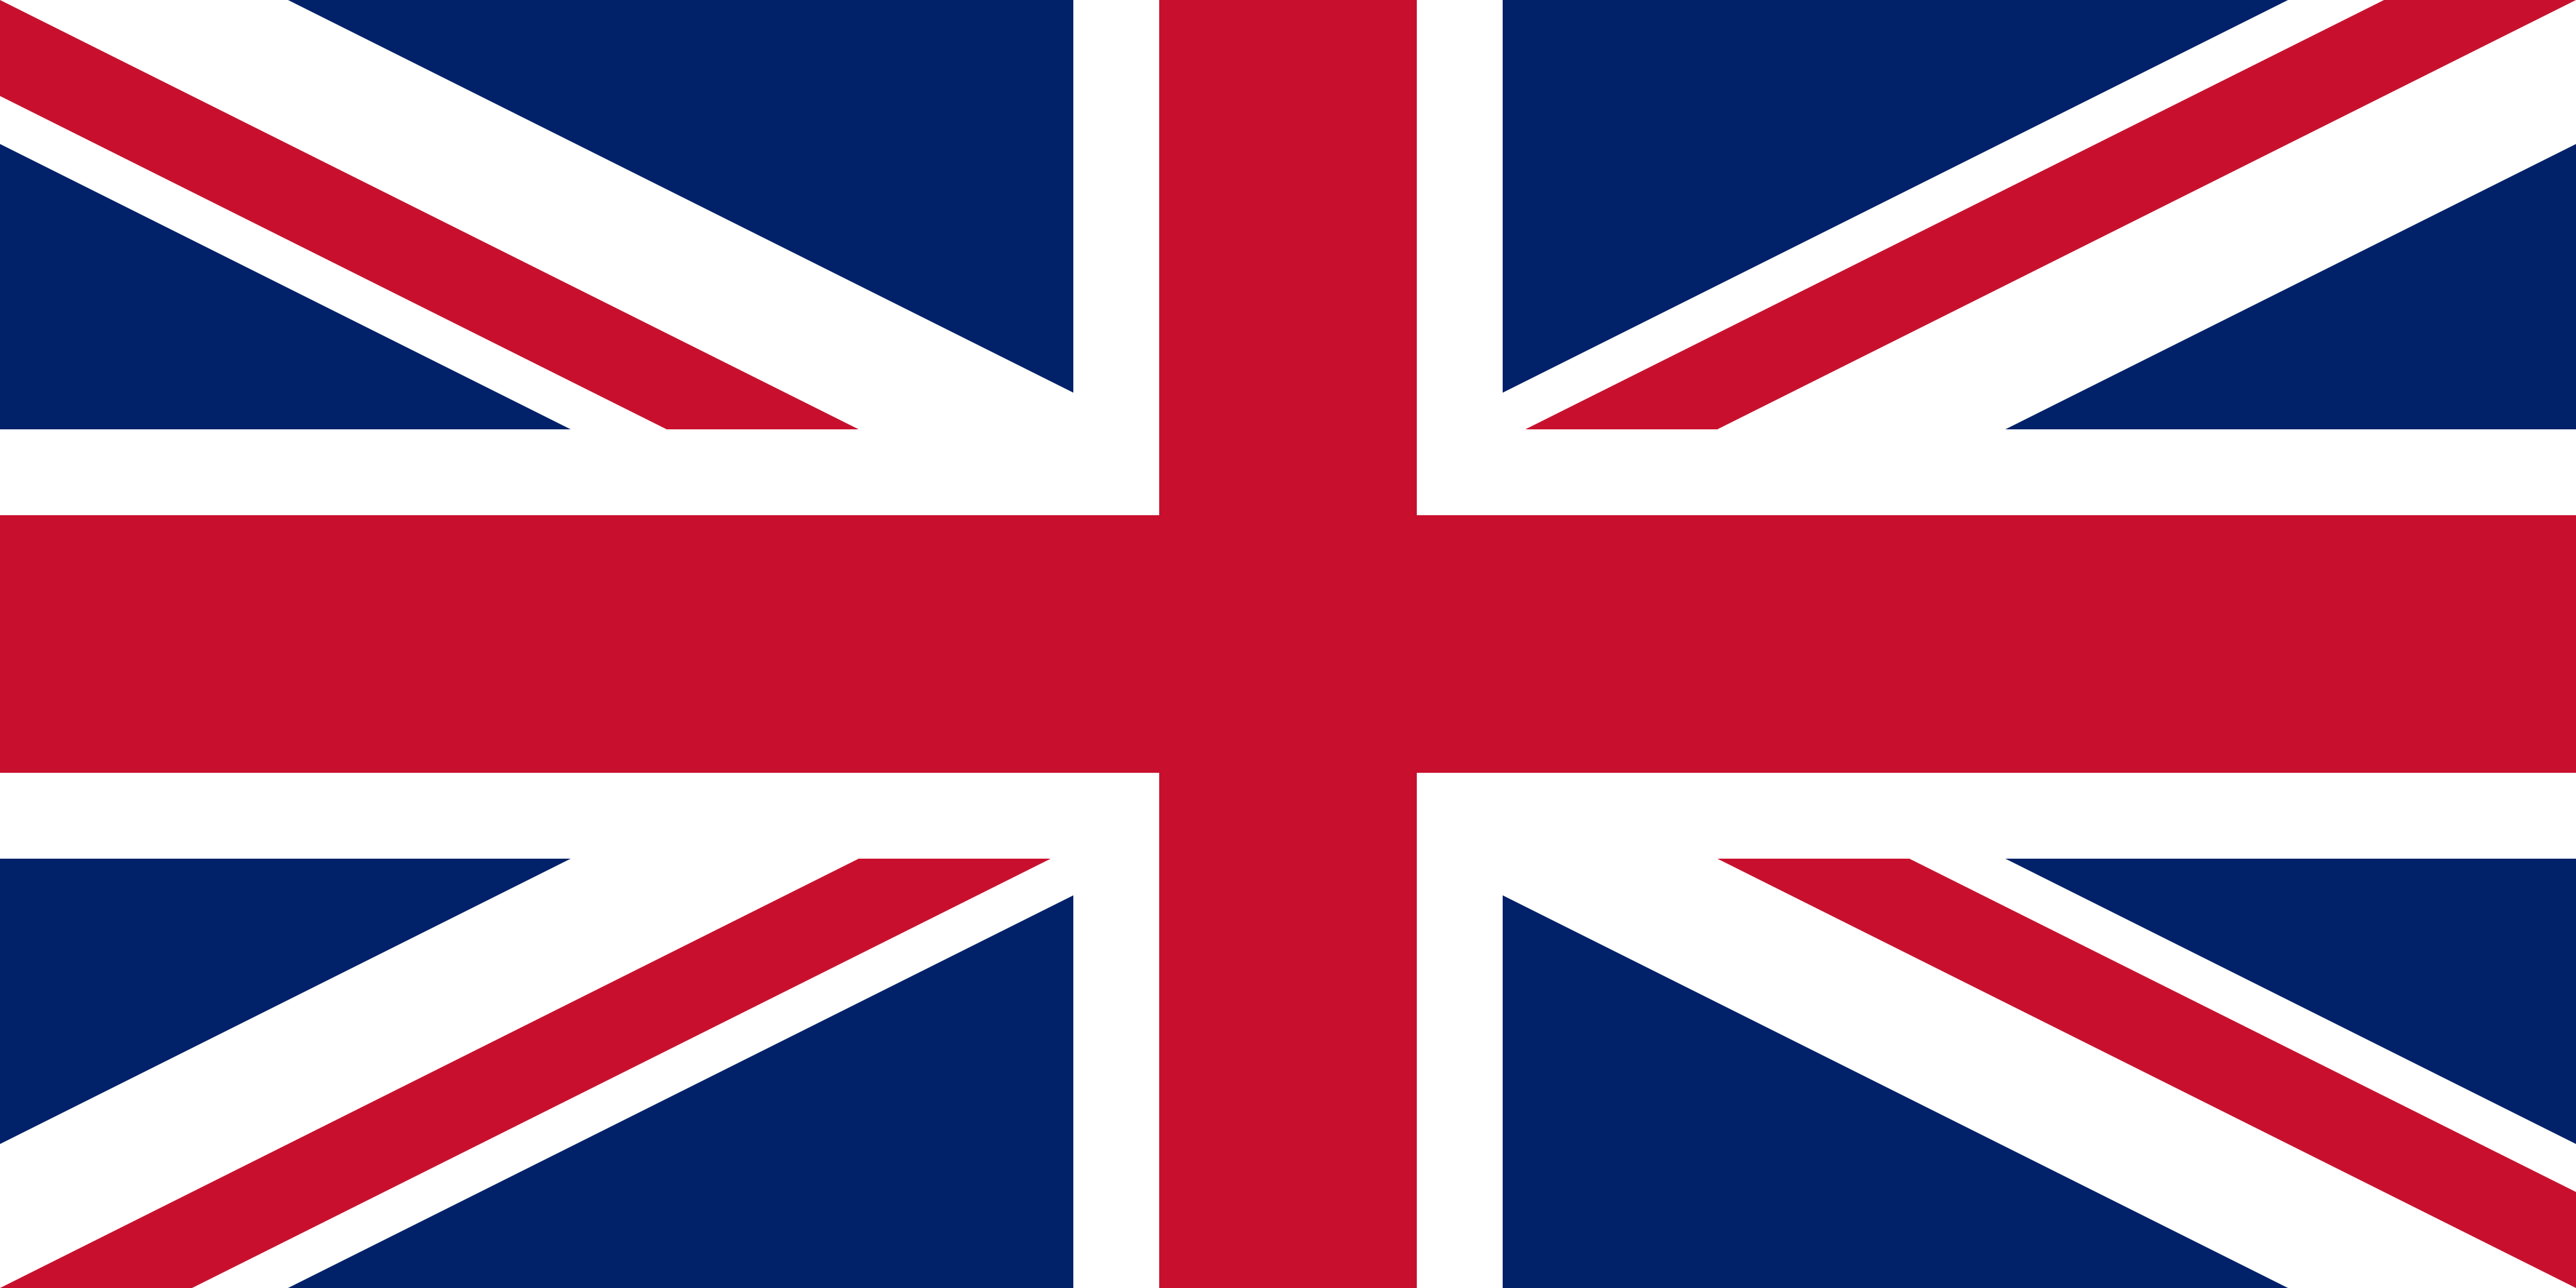
\includegraphics[height=.8em]{uk.png}%
}

\fancypagestyle{firstpage}{
    \fancyhf{}
    \renewcommand{\headrulewidth}{0pt}
    \renewcommand{\footrulewidth}{0pt}
    \fancyfoot[C]{%
        {\setlength{\fboxsep}{7pt}%
        \setlength{\fboxrule}{1.0pt}%
        \fbox{\parbox{0.62\textwidth}{\centering
        \textbf{Forhold mellem krus og drinks-kande}\\
        \large\textbf{1 TIL 3}}}\\[0.35em]
        \footnotesize Ikke på menuen? Mix 4 cl spiritus, 2 cl sirup og en mixer/sodavand
        }
    }
}

\fancypagestyle{secondpage}{
    \fancyhf{}
    \renewcommand{\headrulewidth}{0pt}
    \renewcommand{\footrulewidth}{0pt}
    \fancyfoot[C]{%
        {\setlength{\fboxsep}{7pt}%
        \setlength{\fboxrule}{1.0pt}%
        \fbox{\parbox{0.62\textwidth}{\centering
        \textbf{Cup to pitcher ratio}\\
        \large\textbf{1 TO 3}}}\\[0.35em]
        \footnotesize Not on the menu? Mix anything with 4 cl of spirits, 2 cl syrups and a mixer/soda
        }
    }
}

\backgroundsetup{
    scale=0.4,
    opacity=0.10,
    angle=0,
    contents={
\includegraphics{fredagscafeenlogo.png}}
}

\begin{document}
\thispagestyle{firstpage}

\begin{center}
    \textbf{\LARGE Drinksopskrifter 04-2026 \dkflag }
\end{center}

\vspace{0.1em}

\begin{multicols}{2}

\section*{Champagnebrus}
\begin{itemize}
    \item 4 cl Cuba Caramel
    \item Fyld med 1 Sportsodavand
\end{itemize}

\section*{Filur (Vodka Sunrise)}
\begin{itemize}
    \item 4 cl Vodka
    \item 1 Appelsinjuice
    \item 2 cl Grenadine hældt til sidst
\end{itemize}

\section*{Isbjørn (Blue Lagoon)}
\begin{itemize}
    \item 4 cl Vodka
    \item 1 Sportsodavand
    \item 2 cl Blå Curacao hældt til sidst
\end{itemize}

\section*{Brandbil}
\begin{itemize}
    \item 4 cl Jägermeister
    \item Fyld med 1 Hindbær sodavand
\end{itemize}

\section*{Flügel}
\begin{itemize}
    \item 4 cl rød Eristoff vodka
    \item Fyld med 1 Energidrik
\end{itemize}



\section*{Gin \& Tonic}
\begin{itemize}
    \item 4 cl Gin
    \item Fyld med (Hancock) Tonic
\end{itemize}


\section*{Vodka \& Red Bull}
\begin{itemize}
    \item 4 cl Vodka
    \item Fyld med 1 Red Bull
\end{itemize}


\section*{Kinderægshots}
\begin{itemize}
    \item Kop-sæt (Blandet i krus):
    \begin{itemize}
        \item 12 cl Licor 43
        \item 1 Cocio
        \item 10 shotglas ved siden af
    \end{itemize}
    \item Kande-sæt (Blandet i kande):
    \begin{itemize}
        \item 36 cl Licor 43
        \item 3 Cocio
        \item 10 shotglas ved siden af
    \end{itemize}
\end{itemize}

\columnbreak

\section*{Haribomix}
\begin{itemize}
    \item 2 cl Vodka
    \item 2 cl Cuba Caramel
    \item 1 Appelsin sodavand
    \item 2 cl Grenadine hældt til sidst
\end{itemize}

\section*{Gin Hass}
\begin{itemize}
    \item 4 cl gin
    \item Fyld med 1 lemon sodavand
    \item 2 cl mangosirup hældt til sidst
\end{itemize}

\section*{Tequila Sunrise}
\begin{itemize}
    \item 4 cl Tequila
    \item Fyld med 1 Appelsinjuice
    \item 2 cl Grenadine hældt til sidst
\end{itemize}

\section*{Rum \& Coke}
\begin{itemize}
    \item 4 cl Rom
    \item 1 Cola
    \item En smule Lime- eller Citronsaft
\end{itemize}

\section*{Dark 'n' Stormy}
\begin{itemize}
    \item 4 cl Rom
    \item Fyld med 1 Ginger Beer
    \item En smule Lime- eller Citronsaft
\end{itemize}

\section*{Snigende Gulvtæppe}
\begin{itemize}
    \item (Southern Comfort, Galliano, Gin, Abrikoslikør, Grenadine)
    \item 10 cl Snigende Gulvtæppe premix
    \item Fyld med 1 Sportsodavand
\end{itemize}

\section*{Long Island Iced Tea}
\begin{itemize}
    \item Premix:
    \begin{itemize}
        \item 10 cl Langelænder premix
    \end{itemize}
    \item Eller selvblandet:
    \begin{itemize}
        \item 2 cl Gin
        \item 2 cl Rom
        \item 2 cl Tequila
        \item 2 cl Cointreau
        \item 2 cl Vodka
    \end{itemize}
    \item Fyld med Cola
    \item En smule Lime- eller Citronsaft
\end{itemize}


\end{multicols}

\newpage
\thispagestyle{secondpage}

\begin{center}
    \textbf{\LARGE Drink Recipes 04-2026 \ukflag}
\end{center}

\vspace{0.1em}

\begin{multicols}{2}

\section*{Champagnebrus}
\begin{itemize}
    \item 4 cl Cuba Caramel
    \item Top up with 1 sports soda
\end{itemize}

\section*{Filur (Vodka Sunrise)}
\begin{itemize}
    \item 4 cl Vodka
    \item 1 Orange juice
    \item 2 cl Grenadine poured last
\end{itemize}

\section*{Isbjørn (Blue Lagoon)}
\begin{itemize}
    \item 4 cl Vodka
    \item 1 sports soda
    \item 2 cl Blue Curacao poured last
\end{itemize}

\section*{Brandbil}
\begin{itemize}
    \item 4 cl Jagermeister
    \item Top up with 1 raspberry soda
\end{itemize}

\section*{Flügel}
\begin{itemize}
    \item 4 cl red Eristoff vodka
    \item Top up with 1 energy drink
\end{itemize}


\section*{Gin \& Tonic}
\begin{itemize}
    \item 4 cl Gin
    \item Top up with (Hancock) Tonic
\end{itemize}

\section*{Vodka \& Red Bull}
\begin{itemize}
    \item 4 cl Vodka
    \item Fill with 1 Red Bull
\end{itemize}



\section*{Kinder egg shots}
\begin{itemize}
    \item Cup set (mixed in cup):
    \begin{itemize}
        \item 12 cl Licor 43
        \item 1 Cocio
        \item 10 shot glasses on the side
    \end{itemize}
    \item Pitcher set (mixed in pitcher):
    \begin{itemize}
        \item 36 cl Licor 43
        \item 3 Cocio
        \item 10 shot glasses on the side
    \end{itemize}
\end{itemize}

\columnbreak

\section*{Haribomix}
\begin{itemize}
    \item 2 cl Vodka
    \item 2 cl Cuba Caramel
    \item 1 Orange soda
    \item 2 cl Grenadine poured last
\end{itemize}

\section*{Gin Hass}
\begin{itemize}
    \item 4 cl gin
    \item Top up with 1 lemon soda
    \item 2 cl mango syrup poured last
\end{itemize}

\section*{Tequila Sunrise}
\begin{itemize}
    \item 4 cl Tequila
    \item Top up with 1 orange juice
    \item 2 cl Grenadine poured last
\end{itemize}

\section*{Rum \& Coke}
\begin{itemize}
    \item 4 cl Rum
    \item 1 Cola
    \item A splash of lime or lemon juice
\end{itemize}

\section*{Dark 'n' Stormy}
\begin{itemize}
    \item 4 cl Rum
    \item Top up with 1 Ginger Beer
    \item A splash of lime or lemon juice
\end{itemize}

\section*{Snigende Gulvtæppe}
\begin{itemize}
    \item (Southern Comfort, Galliano, Gin, Apricotliqueur, Grenadine)
    \item 10 cl Snigende Gulvtæppe premix
    \item Top up with 1 sports soda
\end{itemize}

\section*{Long Island Iced Tea}
\begin{itemize}
    \item Premix:
    \begin{itemize}
        \item 10 cl Langelænder premix
    \end{itemize}
    \item Or mixed from scratch:
    \begin{itemize}
        \item 2 cl Gin
        \item 2 cl Rum
        \item 2 cl Tequila
        \item 2 cl Cointreau
        \item 2 cl Vodka
    \end{itemize}
    \item Top up with Cola
    \item A splash of lime or lemon juice
\end{itemize}


\end{multicols}

\end{document}